	\documentclass[]{article}
	\usepackage{tikz}  %TikZ central library is called.
\usetikzlibrary{positioning,shapes,fit,arrows}
\tikzset{set/.style={draw,circle,inner sep=0pt,align=center}}
\usepackage{amssymb} 

%opening
\title{Algebra}
\author{José Guilherme Vanz}

\begin{document}

\maketitle

\section{Numbers}

\subsection{Natural numbers $\mathbb{N}$}

\textit{Natural numbers} ($\mathbb{N}$) start from 1 and goes forever always increasing by 1.

\[ 1,2,3,4,5... 1000, 1000000, ..., \infty\]

Negatives numbers, numbers with decimals, zero are \textbf{not} Natural numbers. For example:

\[ -1,000 \]
\[\frac{1}{3}\]
\[ 89.1 \]

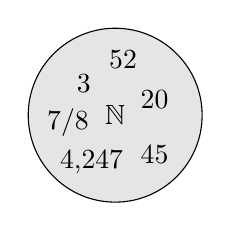
\begin{tikzpicture}
\node[set,fill=gray!20,text width=2.2cm] (nat) at (0,0) {$\mathbb{N}$};
\node[draw=none] at (0.5,0.2) {20};
\node[draw=none] at (0.5,-0.5) {45};
\node[draw=none] at (-0.4,0.4) {3};
\node[draw=none] at (0.1,0.7) {52};
\node[draw=none] at (-0.6,-0.1) {7/8};
\node[draw=none] at (-0.3,-0.6) {4,247};
\end{tikzpicture}

\subsection{Integers}

All number from -$ \infty $ to $ \infty $. They can be written without any fractions or decimals

\[-4, -3, -2, -1, 0, 1, 2, 3, 4\]

\section{Set}

A \textbf{set} is a collection of numbers
A \textbf{subset} is a set of numbers that are all contained in another set

\section{Rational Numbers}

A rational number is a number that can be written as:

\[ \frac{a}{b} \]

where $a$ and $b$ are \textit{integers} and $b$ is different of zero $ b \neq 0$

% I'm not sure if this subsection should be here. But I'll keep it for now
\subsection{Ratio}
In Math a ratio between two numbers indicates how many times the first number contains the seconds. 

\end{document}
